\subsection{Esercizio 7}
Utilizzare le $function$ del precedente esercizio per determinare una approssimazione
della radice della funzione
\[
    f(x) = \left[x - cos(\frac{\pi}{2}x)\right]^3,
\]
per $tol = 10^{-3}, 10^{-6}, 10^{-9}, 10^{-12},$ partendo da $x_0 = 1$
(e $x_1 = 0.99$ per il metodo delle secanti). Tabulare i risultati,
in modo da confrontare le iterazioni richieste da ciascun metodo. Commentare
i risultati ottenuti.
\newline \textbf{Soluzione:} \newline
Eseguendo lo script \nameref{cod:7}si ottengono i risultati contenuti nella tabella \ref{tab:7}
e nella figura \ref{fig:es7}. Come si può notare, il metodo di newton e il metodo delle secanti
convergono molto più rapidamente del metodo di bisezione e del metodo delle corde.
\begin{table}[h]
        \renewcommand\arraystretch{2}
        \begin{tabular}{|l l l l l|}
                \hline
                Metodo     & tolleranza$=10^{-3}$ & tolleranza$=10^{-6}$ & tolleranza$=10^{-9}$ & tolleranza$=10^{-12}$ \\
                \hline
                newton     & 5.94611646360541e-01 & 5.94611644056836e-01 & 5.94611644056836e-01 & 5.94611644056836e-01  \\
                secanti    & 5.94611646954077e-01 & 5.94611644056836e-01 & 5.94611644056836e-01 & 5.94611644056836e-01  \\
                steffensen & 5.94611681141925e-01 & 5.94611644056837e-01 & 5.94611644056836e-01 & 5.94611644056836e-01  \\
                \hline
        \end{tabular}
        \caption{valori approssimati con i metodi di Newton, secanti e Steffensen}
        \label{tab:6}
\end{table}
% \newpage
\begin{figure}[h!]
        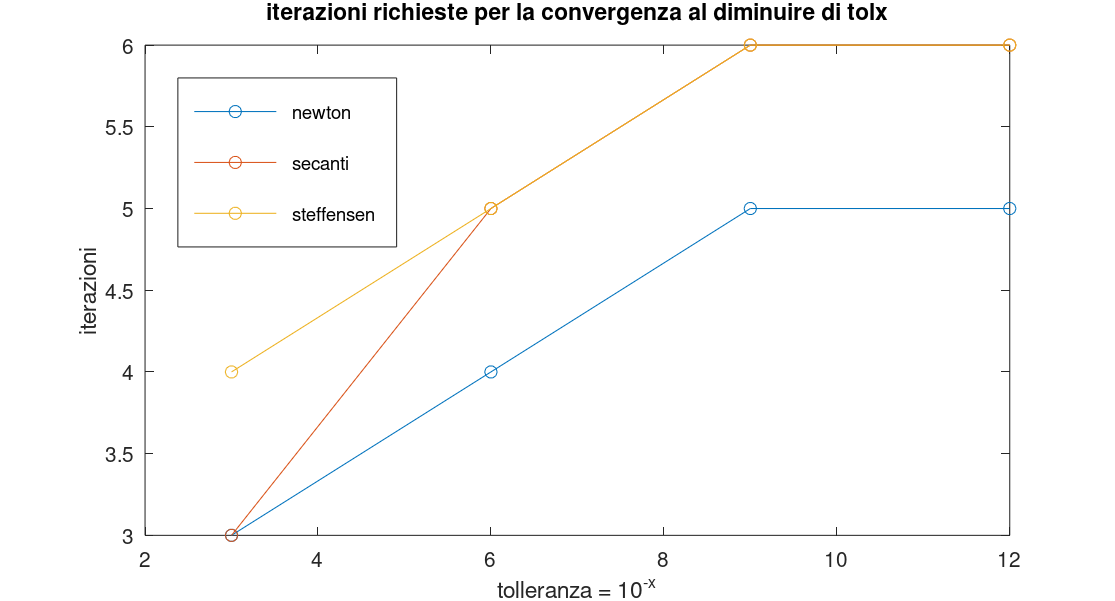
\includegraphics[scale=0.7]{capitolo2/es6_figure.png}
        \caption{iterazioni richieste}
        \label{fig:es7}
\end{figure}
